\documentclass[10pt]{article}

\usepackage{fontspec}
\setsansfont{DejaVu Sans} % Verdana: DejaVu Sans, Cantarell, Open Sans, Droid Sans are all similar, select your preferred
\renewcommand{\familydefault}{\sfdefault}

\usepackage[a4paper, left=1cm, right=1cm, top=1.3cm, bottom=1.17cm]{geometry} % Margins

\usepackage{tabularx} % Tables
\usepackage{array,booktabs} % Table borders
\usepackage{mdframed} % Table spread across multiple pages
\mdfdefinestyle{table}{frametitlerule=true, frametitlefont=\normalfont, frametitlerulewidth=1.5pt, linewidth=1.5pt}

\usepackage{enumitem} % Condensed lists

\usepackage[colorlinks, allcolors=blue, xetex]{hyperref} % URLs

\usepackage{ulem} % Strikethrough

% Header in the first page
\pagenumbering{Alph}
\usepackage{fancyhdr}
\fancyhf{} % clear all header and footer fields
\renewcommand{\headrulewidth}{0pt}
\fancyhead[R]{\rmfamily{2015.01\textbf{\thepage}}}
\pagestyle{fancy}

\usepackage{natbib}
\bibliographystyle{apalike}

\usepackage{graphicx}
\usepackage{caption}

\usepackage{enumitem}

\usepackage{pgfgantt}

\begin{document}

\begin{center}{\large\textbf{PE\&RC PhD PROJECT PROPOSAL}}

\textit{Please read the appendix with instructions first}\end{center}

\noindent\begin{tabularx}{\textwidth}[]{!{\vrule width 1.5pt}X|X!{\vrule width 1.5pt}}
\specialrule{1.5pt}{0pt}{0pt}
\multicolumn{2}{!{\vrule width 1.5pt}l!{\vrule width 1.5pt}}{\textbf{1. GENERAL PROJECT INFORMATION}} \\
\specialrule{1.5pt}{0pt}{0pt}
Main PE\&RC affiliated Institute / University & Wageningen University \& Research\\
\hline
Main PE\&RC research group & Laboratory of Geo-information Science and Remote Sensing\\
\hline
Other PE\&RC groups involved & \\
\hline
Project Title (English) & Large-scale land cover change monitoring from dense time series of satellite data\\
% Alternative titles:
% Towards a global land cover change monitoring system: consistency and expressing reality via class fractions.
% Global land cover change mapping: improving methods and ways to express reality with class fractions.
% Global land cover change mapping: feasibility and expressing reality via class fractions.
\hline
Project duration & FROM 01/11/2017 TO 31/10/2021\\
\hline
Where will the research be conducted (country) & Netherlands\\
\hline
At which University will the thesis be defended? & Wageningen University \& Research\\
\hline
Funding source(s) for this project (1, 2, or 3?) & \sout{1 (internal) / 2 (NWO) /} 3 (external) (strikethrough)\\
\hline
Name of funding source: & European Commission\\
\specialrule{1.5pt}{0pt}{0pt}
\end{tabularx}

\bigskip

\noindent\begin{tabularx}{\textwidth}[]{!{\vrule width 1.5pt}X|X!{\vrule width 1.5pt}}
\specialrule{1.5pt}{0pt}{0pt}
\multicolumn{2}{!{\vrule width 1.5pt}l!{\vrule width 1.5pt}}{\textbf{2. THE PhD CANDIDATE}} \\
\specialrule{1.5pt}{0pt}{0pt}
Full name of the PhD candidate & Dainius Masiliūnas\\
\hline
Gender & MALE \sout{/ FEMALE}\\
\hline
Nationality & Lithuanian\\
\hline
Date of birth & 07/04/1993\\
\hline
Period of appointment & FROM 01/11/2017 TO 31/10/2021\\
\hline
Hours per week & 40\\
\specialrule{1.5pt}{0pt}{0pt}
\end{tabularx}

\bigskip

\noindent\begin{tabularx}{\textwidth}[]{!{\vrule width 1.5pt}X|X|X|X|X!{\vrule width 1.5pt}}
\specialrule{1.5pt}{0pt}{0pt}
\multicolumn{5}{!{\vrule width 1.5pt}l!{\vrule width 1.5pt}}{\textbf{3. SUPERVISION}} \\
\specialrule{1.5pt}{0pt}{0pt}
\textbf{Project role} & \textbf{Name + title} & \textbf{Specialisation} & \textbf{Organisation} & \textbf{Hours/week} \\
\hline
Promotor & Prof. Martin Herold & Global forest and land monitoring & Wageningen University \& Research & 0.25\\
\hline
Co-promotor & Dr Jan Verbesselt & Satellite time series analysis & Wageningen University \& Research & 0.5\\
\hline
Daily supervisor & Dr Nandin-Erdene Tsendbazar & Land cover change analysis and validation & Wageningen University \& Research & 0.5\\
\hline
Advisor & Dr Devis Tuia & Machine learning algorithms in remote sensing & Wageningen University \& Research & As needed\\
\hline
Other &  &  &  & \\
\specialrule{1.5pt}{0pt}{0pt}
\end{tabularx}

\bigskip

\noindent\begin{tabularx}{\textwidth}[]{!{\vrule width 1.5pt}p{4.8cm}|X|X!{\vrule width 1.5pt}}
\specialrule{1.5pt}{0pt}{0pt}
\multicolumn{3}{!{\vrule width 1.5pt}l!{\vrule width 1.5pt}}{\textbf{4. COLLABORATION}} \\
\specialrule{1.5pt}{0pt}{0pt}
\textbf{Type of organisation} & \textbf{Name of organisation} & \textbf{Name + title of collaborator(s)} \\
\hline
University & \begin{minipage}[t]{\linewidth}\begin{enumerate}[nosep,after=\strut] \item University of Münster (WWU) \end{enumerate}\end{minipage} & Prof. Dr Edzer Pebesma\\
\hline
Research Institute & \begin{minipage}[t]{\linewidth}\begin{enumerate}[nosep,after=\strut] \item Flemish Institute for Technological Research (VITO) \item International Institute for Applied Systems Analysis (IIASA) \end{enumerate}\end{minipage} & Bruno Smets, Myroslava Lesiv\\
\hline
Government agency &  &  \\
\hline
Others (e.g., FAO,WHO) & \begin{minipage}[t]{\linewidth}\begin{enumerate}[nosep,after=\strut] \item OpenEO Consortium \end{enumerate}\end{minipage} & Prof. Dr Wolfgang Wagner \\
\specialrule{1.5pt}{0pt}{0pt}
\end{tabularx}

\bigskip

\noindent\begin{tabularx}{\textwidth}[]{!{\vrule width 1.5pt}X|p{4.5cm}!{\vrule width 1.5pt}}
\specialrule{1.5pt}{0pt}{0pt}
\multicolumn{2}{!{\vrule width 1.5pt}l!{\vrule width 1.5pt}}{\textbf{5. ETHICS}} \\
\specialrule{1.5pt}{0pt}{0pt}
Will vertebrates be used in animal experiments? & \sout{YES /} NO\\
\hline
Are there other ethical issues to be considered with respect to this project? & \sout{YES /} NO\\
\hline
\multicolumn{2}{!{\vrule width 1.5pt}l!{\vrule width 1.5pt}}{If YES, please elaborate:}\\[1cm]
\specialrule{1.5pt}{0pt}{0pt}
\end{tabularx}

\newpage

\begin{center}{\large\textbf{PE\&RC PhD PROJECT PROPOSAL}}

\textit{In case a peer-reviewed full project proposal is available (e.g., NWO or EU), please send that proposal along together with the reviewers comments and the acceptance letter.}\end{center}

\begin{mdframed}[style=table,frametitle=\textbf{6. SUMMARY} (max. 250 words)]
%Importance of land cover change detection, potential users

%Summary of the four objectives
Land cover is essential for a wide variety of users, ranging from land owners to national governments to the scientific community for modelling climate change. Monitoring the change in land cover allows stakeholders to take informed decisions about how to control their land, and allows scientists to use more accurate models that take land variability into account.

In this project, the methods for creating and updating land cover change products will be improved by: 1) performing fractional land cover mapping in order to better express the reality on the ground, such as gradual land cover change, more precisely; 2) improving the reliability of temporal features obtained from remote sensing imagery time series by detecting breaks in the time series; 3) investigating land cover map updating methods to reduce spurious changes between annual land cover maps; 4) deriving land cover change products from fractional land cover data. The combination of these methods will allow for a more consistent and accurate representation of land cover changes happening through time at a global scale.
\end{mdframed}

\begin{mdframed}[style=table,frametitle=\textbf{7. DETAILED DESCRIPTION OF THE RESEARCH PLAN} (max. 2500 words + 1 page literature list)]
\section{Introduction}
Land cover is an essential variable that describes the state of the land at a given point in time. It is important to a variety of users: due to its practical meaning and ease of deriving statistics, it is important for national governments and NGOs, as well as to individual land owners. It is also a key variable for to scientists, that attempt to model global processes, ranging from local air quality to global climate change; indeed, land cover has been identified as an Essential Climate Variable by the Global Climate Observing System, and is important for monitoring a number of sustainable development goals defined by the United Nations.

At the moment, a number of global land cover maps exist: GLC2000, based on the SPOT-4 VEGETATION sensor at 1 km resolution \citep{bartholome_glc2000:_2005}; MODIS yearly land cover maps at 500 m resolution \citep{friedl_modis_2010}; GlobCover 2005 and 2009, based on the MERIS sensor at 300 m resolution \citep{arino_globcover:_2007}; Land Cover CCI, based on both MERIS and SPOT4 VEGETATION at 300 m resolution \citep{bontemps_consistent_2013} and GlobeLand30, based on Landsat sensors at 30 m resolution \citep{chen_global_2015}. However, these maps only describe the land cover for a particular year, and are updated infrequently, only once in a few years.

While it is important to know the land cover type of a particular area, most applications are rather focused on land cover dynamics, i.e. what part of land cover changed over a period of time. This information is important for national monitoring programmes, as well as for scientific models, whose goal is to predict change in the future. While it is possible to obtain information about land cover change by differencing two yearly land cover maps (such as those of MODIS), it leads to higher errors: the errors of both land cover maps propagate into the created land cover change map. That way, spurious changes due to the sensitivity of the land cover prediction model to small changes in input variables (rather than to actual changes on the ground) show up, but are false positives. Given that current global land cover maps have an accuracy of approximately 70\% \citep{bontemps_revisiting_2012}, the resulting land cover change map is even less accurate. There have been initiatives to update land cover maps by using more advanced techniques than differencing, such as by employing break detection between images to only update the land cover in pixels that have changed \citep{jin_land_2017}, however, these techniques increase the rate of false negatives by assuming that all pixels without detected breaks have not changed since the previous time step.

Another property that all of the aforementioned global land cover maps share is that each pixel is said to belong to a certain land cover class; the classification is based on classes with \textit{discrete} labels. In reality, land cover does not follow a grid pattern, and a large proportion of pixels in a moderate resolution remote sensing image cover an area that includes more than a single land cover class. This is a problem especially in heterogeneous areas with small patch sizes. Classification with discrete labels can only express the dominant land cover type in a pixel, any information about other land cover types in the same pixel is lost. In contrast, producing a map of \textit{fractions} of land cover classes allows for expressing the proportion of each land cover class in each pixel, which in turn eliminates the need for mosaic classes and makes the legend easier to interpret. Fractional land cover maps can also be reduced to discretely labelled maps, allowing users to define their own rules and thresholds for doing so, thus taking into account which classes the user is interested in \citep{tsendbazar_integrating_2017}. In addition, coarser resolution fractional land cover mapping reduces the uncertainty of classification, since the requirement of knowing the specific location of a particular land cover class is relaxed. This addresses the needs of the scientific community, where models do not require high spatial resolution, but require higher accuracy \citep{bontemps_revisiting_2012}.

Fractional classification (also known as fuzzy classification) has been popular in the past, when only coarse resolution imagery was available \citep{foody_approaches_1996, adams_classification_1995, amo_spectral_2002}. In recent years, fractional classification has been gaining support once again, as a method to better represent land cover \citep{gessner_estimating_2013}, but the suitability for global land cover mapping as well as the issue of updating fractional land cover maps has been largely unexplored up to now. Current global land cover products only include cover fractions for specific land cover classes, such as forests \citep{hansen_global_2003}, rather than covering the full range of land cover classes, and they do not yet distinguish between different tree cover types.

%New global land cover maps with a high resolution and frequent updating are emerging and Land Cover CCI, based on the Sentinel-2 MSI sensor at 20m resolution.
%Global land cover classification maps: importance and existing products, use cases and shortcomings

%Land cover change products (yearly/continuous) and initiatives to update land cover classification maps, challenges \citep{bontemps_revisiting_2012}

%Fuzzy vs hard classification

%Potential of global fuzzy classification maps and fuzzy land cover change: user-generated maps, consistency in model parameters, lower uncertainty, less data to process, transitions are more true to the processes on the ground, possibility to derive hard maps

\centerline{
  \begin{minipage}[t]{0.8\linewidth}
    %\vspace{-2ex}
    \bigskip
    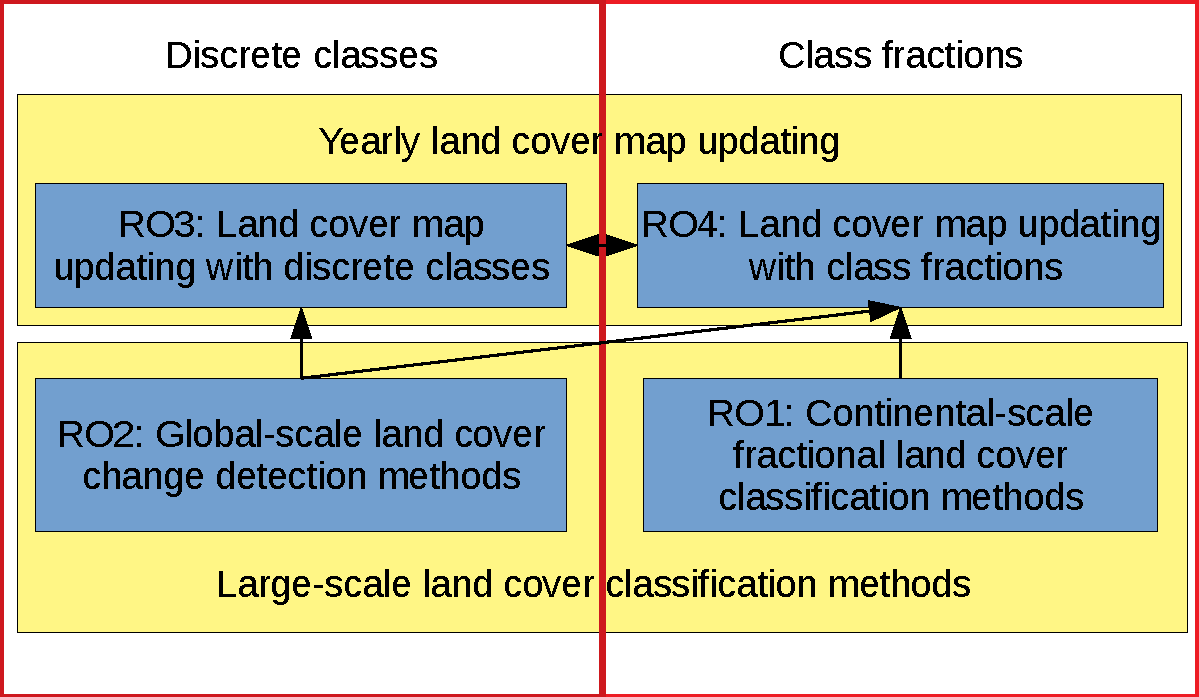
\includegraphics[width=\linewidth]{figures/objectives.pdf}
    \captionof{figure}{Research objectives and their relations. The first two objectives form the base of the research and investigate the methods for performing large-scale land cover classification (lower yellow box). The last two objectives concern updating land cover maps (upper yellow box). The research questions are divided into methods and map updating when using discrete classes (left box) and when using class fractions (right box).}
    \label{fig-objectives}
  \end{minipage}
}

\section{Research challenges and hypotheses}
This research project aims to address the following research challenges:

\begin{enumerate}
 \item There is a variety of machine learning algorithms that are able to produce information about the fractions of land cover classes, but some are not suitable for continental or global scale classification due to their computational intensity, low accuracy (overfitting), and/or ability to deal with non-normal or collinear variables.
 \item Extracting temporal features from time series of satellite data without consideration of land cover change occurring during the time period leads to the temporal metrics being a mix between several land cover classes. Break detection in time series can be used to detect periods of stable land cover.
 \item Differences between land cover maps produced annually are often spurious, rather than reflecting actual changes on the ground. This issue can be eliminated by making the methods of producing the maps more conservative, rather than presuming that either of the two maps is error-free.
 \item Discrete land cover classes cannot express gradual changes from one class to another, only abrupt changes affecting an entire pixel. Using class fractions would allow for expressing such changes.
\end{enumerate}

These points also serve as hypotheses for the research objectives listed below.

\section{Research objectives}

The aim of this PhD project is to develop methods for global scale land cover classification, change detection and map updating for both discrete and fractional land cover classes. In order to achieve this aim, the project is subdivided into four research objectives:

\begin{enumerate}[label=RO\arabic*]
 \item \label{RO1} To compare the suitability of machine learning algorithms for performing continental-scale fractional land cover mapping.
 \item \label{RO2} To improve the robustness of time series-derived temporal metrics used in land cover mapping by performing land cover change detection on dense time series.
 \item \label{RO3} To compare methods for creating annually consistent and stable global land cover change maps with discrete class labels. % And error propagation/uncertainty?
 \item \label{RO4} To investigate the methods of representing land cover changes between years using a set of fractional land cover maps.
\end{enumerate}

The objectives and their relations are visualised in figure \ref{fig-objectives}.

\section{Research methodology}
\subsection{Continental-scale fractional land cover classification method comparison}
\centerline{
  \begin{minipage}[t]{0.69\linewidth}
    %\vspace{-2ex}
    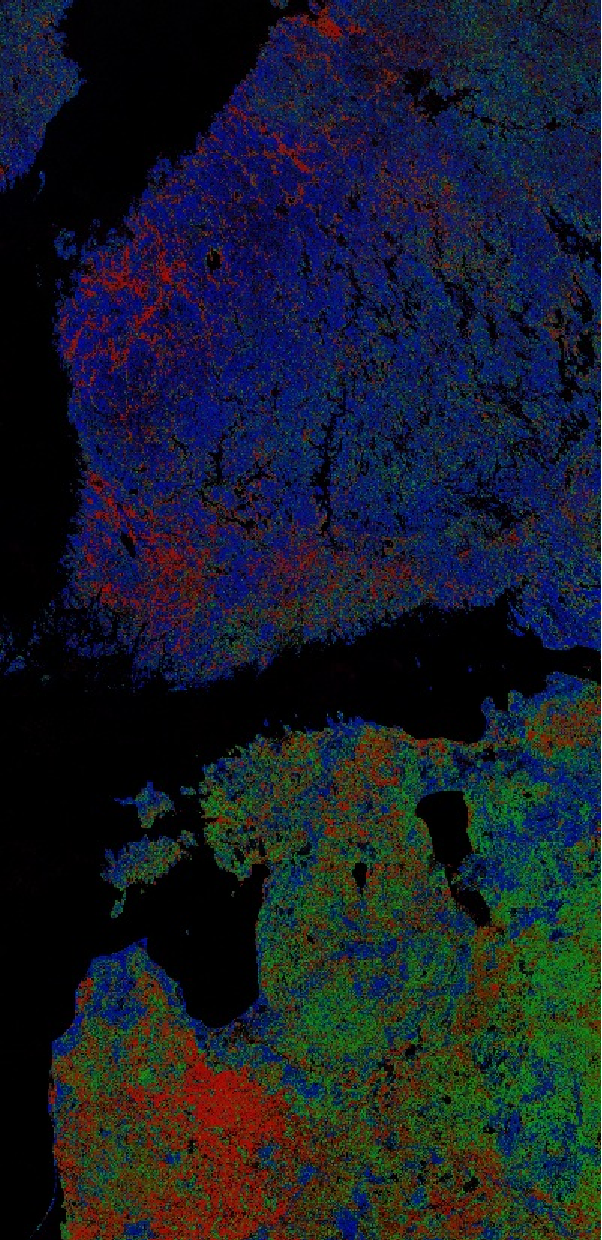
\includegraphics[width=0.5\linewidth]{figures/fulltile-rf.pdf}
    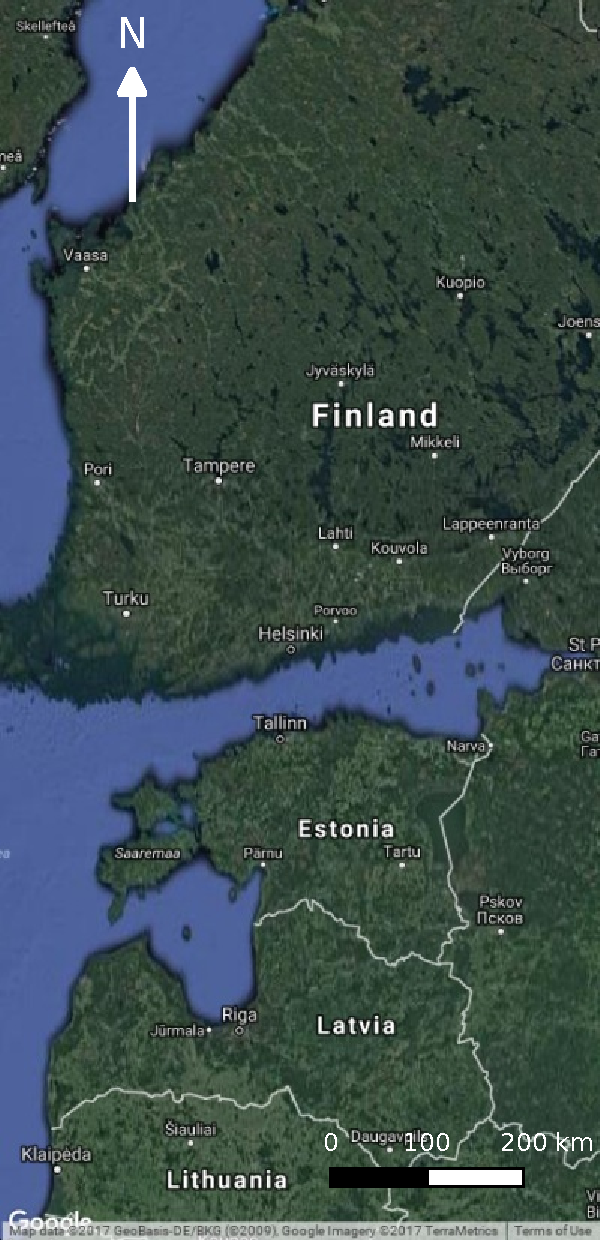
\includegraphics[width=0.5\linewidth]{figures/fulltile-google.pdf}
    \captionof{figure}{Fractional land cover classification of the area between the middle of Lithuania and Finland. Left: land cover fractions mapped to RGB channels (red: agriculture, green: deciduous trees, blue: evergreen trees). Right: true colour Google Imagery of the area.}
    \label{fig-fractional-tile}
    \bigskip
  \end{minipage}
}

The aim of \ref{RO1} is to compare machine learning methods for fractional land cover classification over the continent of Africa and a case study in Europe (see figure \ref{fig-fractional-tile}). For fractional classification, methods used for discrete label classification are often not suitable, as they only provide a label of the most likely class at the pixel, rather than performing a regression and providing the fraction of each class in a pixel.

Nevertheless, there are several machine learning algorithms that are capable of producing fractional output per category, such as supervised fuzzy \textit{c}-means \citep{hengl_double_2004} and neural networks \citep{foody_fully_1997}. In addition, regression methods such as random forest regression \citep{breiman_random_2001} can be used to provide estimates of each land cover fraction independently, and then be combined into a unified map with a post-procesing step. These methods will be tested in order to assess the output map accuracy both visually and statistically, as well as to assess the computing time required for each method in order to determine the suitability of each method for performing global land cover classification.

These methods will be applied on time series data derived from the PROBA-V satellite archive (100 m resolution imagery at the equator) over the continent of Africa, and one case study site in Europe in order to test the applicability of the methods to a boreal forest gradient. Auxiliary data will also be included to serve as extra information for deriving the land cover fractions. The algorithms will be trained and validated on land cover sampling data that has been collected as part of the Copernicus Global Land Operations ``Vegetation and Energy'' (CGLOPS-1) project (see figure \ref{fig-sampling-fractions}, over 25000 sampling points over Africa in separate training and validation sets). Processing will be carried out on the Proba-V Mission Exploitation Platform (MEP), which allows direct access to Proba-V satellite imagery.

This objective forms a basis for \ref{RO4}, where the most suitable method from the ones tested in \ref{RO1} will be used in order to create fractional land cover maps for different years and derive a map of land cover changes over time.

\subsection{Land cover classification guided by time series break detection}

\centerline{
  \begin{minipage}[t]{0.9\linewidth}
    %\vspace{-2ex}
    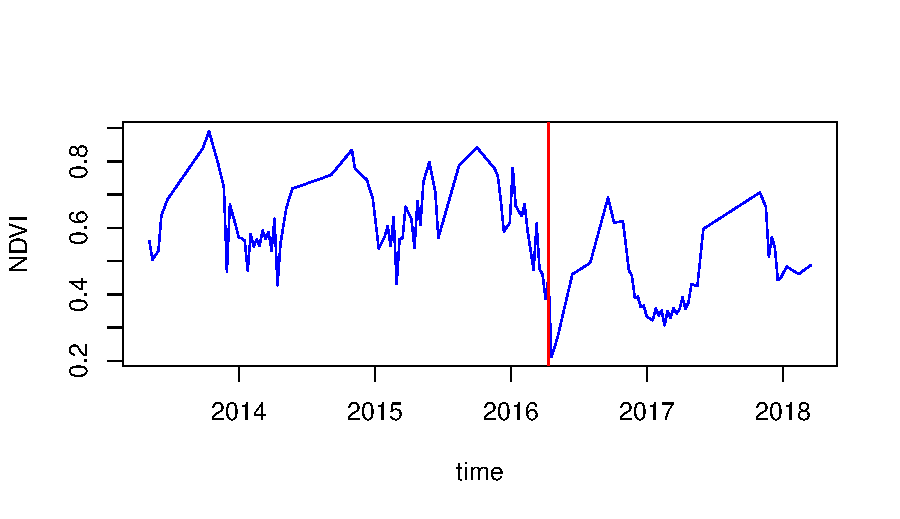
\includegraphics[width=\linewidth]{figures/guinea.pdf}
    \captionof{figure}{Landsat-based NDVI time series of a forest in Guinea that underwent changes in 2016. Detecting the break (break detected using the \texttt{strucchange} package indicated in red) allows for extracting temporal features only from periods of stable land cover: from 2013 up to the break, and from the break to the present day. This is most important for classifying the land cover of this pixel in 2016, as without break detection the temporal features would be mixed between two different land cover types.}
    \label{fig-guinea-break}
    \bigskip
  \end{minipage}
}

The aim of \ref{RO2} is to test the suitability of methods and different input data for detecting land cover changes from time series-derived information. Different land cover classes tend to have distinct time series profiles (e.g. seasonality, phenology), and transitions between the classes cause an abrupt change in these parameters. Detecting such breaks in the time series (see figure \ref{fig-guinea-break}) serves a dual purpose: the land cover in the time in between two breaks may be considered to be stable; and knowing the time of the break allows for deriving temporal metrics only from the part of the time series that is stable. This allows for making the most out of the time series information: in case there is a break, statistics are derived only from the part of the time series that was stable, rather than deriving it from the full time series and getting a mixed response from different land cover types that were present at the location during different times; and if there was no break, then the temporal metrics can be derived from the full time series, making them more robust to issues such as cloud contamination.

There is a variety of methods for detecting breaks in time series, ranging from simple ANOVA applications to models based on structural change theory \citep{bai_least_1994, zeileis_testing_2003}. New methods based on multivariate analysis are also being proposed \citep{lu_spatio-temporal_2016}. Their suitability for the problem of land cover classification at a global scale may vary. In addition, it is important to test how these methods perform on different input data (varying spatial and temporal resolutions from different sensors), including time needed to process a time series, in order to be able to assess how suitable these methods are for global land cover classification.

In order to validate the detection of breaks in time series, additional validation data on land cover change will be collected by the CGLOPS-1 project. This data will include information on whether and at which time there was a change in land cover in a sampling pixel. Sampling stratification will be based on an initial run of the \texttt{strucchange} break detection algorithm \citep{zeileis_testing_2003}, using MODIS data (10-daily EVI composites). The resulting validation dataset will then be used to fine-tune the break detection algorithm, and run it on higher spatial resolution Proba-V, Landsat 7 and Landsat 8 imagery. Data analysis for this objective will also be carried out on the Proba-V MEP.

This objective forms a basis for both \ref{RO3} and \ref{RO4}, in order to derive higher quality temporal metrics from time series data, as well as to serve as an input for testing whether it is sufficient to make use of break detection in order to update land cover maps.

\subsection{Land cover change mapping based on discrete classes}
The aim of \ref{RO3} is to investigate methods for updating land cover maps, focusing on ones with discrete labels. There are two major ways to update land cover maps in use at the moment: rerunning the same model as used to generate the previous land cover map, but using data from the year of interest instead (e.g. \citet{friedl_modis_2010}); and using land cover change detection algorithms in order to only update the pixels where a change has been detected (e.g. \citet{jin_land_2017}). Both of the methods have drawbacks: the former results in spurious changes (false positives) in pixels that have high uncertainty or are composed of a similar proportion of two land cover classes, whereas the latter makes an assumption about the accuracy of the first land cover map and introduces additional uncertainty from the change detection step.

For this objective, the two methods will be compared to one another, and new methods will be proposed and tested against the aforementioned ones. One new method that will be investigated for improving the stability of land cover maps is to make the machine learning model for generating the next land cover map more conservative by also providing it with data on the previous land cover maps of the same area. That way, the model would only produce changes in the updated map if there is significant evidence for change. In the second proposed method, land cover will be updated based on the model uncertainty for each pixel every year: if the uncertainty (and thus confusion) is high between two possible classes at both time steps, the pixel will be considered to be unchanged, and assigned to the class with highest probability at both time steps.

These methods will also be compared to Markov Random Fields, which is a post-classification technique for reducing changes in labels. It takes both the spatial and temporal variability around each pixel into account and can use rules to define how easily a class may transition to another given class. This approach is used in some existing land cover maps (e.g. \citet{cai_enhancing_2014}).

The accuracy of the resulting land cover change maps will be assessed by taking into account both the accuracy of the land cover classification itself the year before and the year after (data as in figure \ref{fig-sampling-fractions}, but discretised rather than fractional), and whether the change has been detected correctly or not by making use of the land cover change validation dataset from \ref{RO2}. The Proba-V MEP cluster will be used to speed up computations.

In this objective, the difference between producing updated land cover maps and producing a separate land cover change map will also be considered. According to user requirement studies \citep{bontemps_revisiting_2012, herold_towards_2016}, both types of maps may be useful for different applications: a land cover map for a particular year represents the best estimation of land cover for that moment in time, whereas a land cover change map is much more conservative than a simple difference map between the years in order to highlight only those areas where there is a high certainty that land cover has in fact changed.

This objective serves as a basis for \ref{RO4}, which deals with the same problem but with class fractions, instead of discrete classes.

\subsection{Land cover change mapping based on class fractions}

\centerline{
  \begin{minipage}[t]{0.9\linewidth}
    %\vspace{-2ex}
    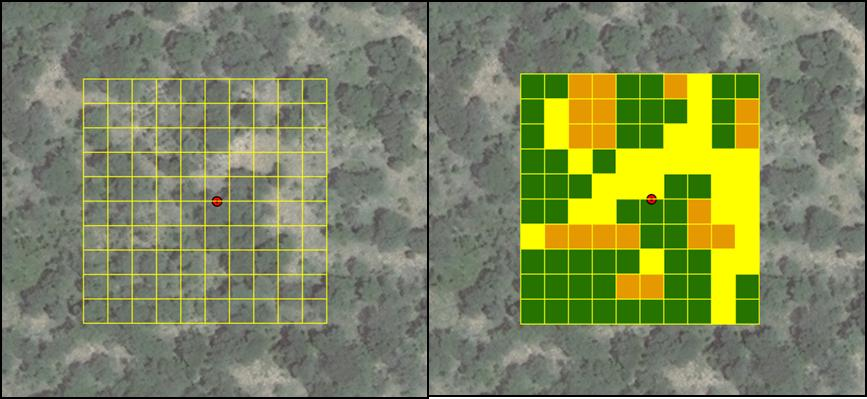
\includegraphics[width=\linewidth]{figures/sampling-fractions}
    \captionof{figure}{Screenshot from an interpretation of a sampling pixel \citep{tsendbazar_validation_2018}. An area covering a Proba-V pixel (nominally 100×100 m) is subdivided into smaller polygons (nominally 10×10 m). These polygons are interpreted by an expert to obtain fractional land cover validation data for each pixel. The acquisition date of the imagery used for interpretation is recorded as well. Over 68000 such sampling pixels have been interpreted globally so far as part of the Copernicus Global Land Operations ``Vegetation and Energy'' (CGLOPS-1) project.}
    \label{fig-sampling-fractions}
    \bigskip
  \end{minipage}
}

The aim of \ref{RO4} is to investigate methods for updating land cover maps that consist of class fractions, rather than discrete classes. Fractional data differs from class label data in its representation, allowing class transitions to be expressed as gradual change in class fractions, rather than an abrupt change from one class to another. This type of representation is closer to reality, where class transitions may happen either abruptly (e.g. deforestation) or gradually (e.g. forest regrowth). However, the traditional methods for expressing changes between yearly maps are not suitable for fractional data, and thus new methods need to be developed, based on user needs.

With discrete classes, one of the challenges of expressing change is that there is the possibility of change between any pair of classes (from-to), leading to a high number of possible combinations. With fractional classes, the transitions are not only between classes, but also the fraction of each class in each pixel. One way to represent change with fractional classes is to display the change in class fraction of each class separately. This is suitable for hotspot analysis to detect areas undergoing fast changes for a class of interest. However, this method may not be suited for monitoring class transitions, as it is not evident which other classes have increased or decreased in their fractions to account for the fraction change in the class of interest. In this case, applying thresholds of change and logical class transitions (e.g. \citet{cai_enhancing_2014}) may allow making use of fractional data to also express class transitions in an easy-to-understand fashion. In addition, visualising the fractions of more than three classes at a time \citep{hengl_double_2004} is challenging, but important for map usability. As a result, more than one type of land cover change map could be produced out of fractional land cover data, depending on the needs of the users. Within this objective, such methods of representing land cover change by making use of fractional land cover data will be investigated.

Validation methods for fractional land cover change will be investigated as well. Using the sampling pixel validation data from the CGLOPS-1 project (figure \ref{fig-sampling-fractions}), root mean square error and related statistics can be used to determine the accuracy of land cover at a particular date. The land cover change validation dataset from \ref{RO2} will be used to validate the detection of large, sudden changes in land cover fractions. The processing for this step will also be carried out on the Proba-V MEP.

\section{Innovative aspects}

In \ref{RO1}, the use of multiple machine learning techniques for fractional land cover mapping at a scale larger than that of a city has not been explored yet. For performing global-scale mapping, the speed of each method is also an important consideration. In \ref{RO2}, multiple break detection methods exist, but there is no comprehensive comparison between them, nor a suitability analysis for a global classification use case. In \ref{RO3}, new methods are proposed to handle cases of spurious land cover changes between maps (false positives) without making an assumption about the accuracy of either one of the maps being compared; these method will be compared to the current practices. In \ref{RO4}, the topic of land cover map updating using fractional land cover classes has scarcely been explored so far altogether, due to the currently used methods for updating discretely classified maps not being applicable to fractional ones, and relatively few land cover maps including fraction information so far. Here, new ways to represent changes in land cover using fractional data will be proposed.

\bibliography{proposal}
\end{mdframed}

%\newpage

\begin{mdframed}[style=table,frametitle=\textbf{8. TIME TABLE OF THE PROJECT AND WORK PROGRAMME}]
%\resizebox{0.7\textwidth}{!}{
\centerline{
    \begin{ganttchart}[hgrid, vgrid, y unit chart=0.9cm]{1}{16}
      \gantttitle{{\tiny 2017}}{1} \gantttitlelist{2018,...,2020}{4} \gantttitle{2021}{3} \\
      \gantttitle[title label node/.append style={below left=-7pt and -6pt}]{Quarters:\quad4}{1} \gantttitlelist{1,...,4}{1} \gantttitlelist{1,...,4}{1} \gantttitlelist{1,...,4}{1} \gantttitlelist{1, ..., 3}{1} \\
      \ganttbar{TSP and proposal writing}{1}{3} \\
      \ganttgroup{Research objective 1}{3}{5} \\
      \ganttbar{Fractional mapping over Africa}{3}{5} \\
      \ganttbar{Paper writing (RO1)}{4}{5} \\
      \ganttgroup{Research objective 2}{2}{7} \\
      \ganttbar{Breakpoint detection}{2}{3} \ganttbar{}{6}{7} \\
      \ganttbar{Paper writing (RO2)}{6}{7} \\
      \ganttgroup{Research objective 3}{4}{10} \\
      \ganttbar{Land cover change modelling, discrete}{4}{4} \ganttbar{}{8}{10} \\
      \ganttbar{Paper writing (RO3)}{9}{10} \\
      \ganttgroup{Research objective 4}{11}{14} \\
      \ganttbar{Land cover change modelling, fractional}{11}{14} \\
      \ganttbar{Paper writing (RO4)}{13}{14} \\
      \ganttgroup{Thesis finalisation}{14}{16} \\
      \ganttbar{Synthesis}{14}{15} \\
      \ganttmilestone{Thesis defence}{16}
    \end{ganttchart}
}
%}
\end{mdframed}

\begin{mdframed}[style=table,frametitle=\textbf{9. SOCIETAL RELEVANCE}]
The outcomes of this PhD project will directly benefit the creation of global land cover and land cover change maps by enhancing their accuracy and versatility. Fractional land cover maps allow the users to define their own classes of interest, adjusting them to their own requirements. This is especially important given the wide variety of users for land cover and land cover change maps. They include national governments for monitoring the land cover of their country, individual large stakeholders for monitoring their concessions, and the scientific community for modelling changes to the Earth system, e.g. climate (as an Essential Climate Variable), forest change, urban development, etc. Improving land cover and land cover change for the entire globe also furthers the Sustainable Development Goals (SDGs) of the United Nations.
\end{mdframed}

\begin{mdframed}[style=table,frametitle=\textbf{10. DATA MANAGEMENT} (max. 250 words)]
Data used and produced within this PhD project will be handled by following the Data Management Plan (DMP) of the Laboratory of Geo-Information Science and Remote Sensing (GRS). The DMP will be prepared as a separate document to describe data handling in more detail.
\end{mdframed}

\newpage

\noindent\begin{tabularx}{\textwidth}[]{!{\vrule width 1.5pt}p{1cm}|X|X|X|X!{\vrule width 1.5pt}}
\specialrule{1.5pt}{0pt}{0pt}
\multicolumn{5}{!{\vrule width 1.5pt}l!{\vrule width 1.5pt}}{\textbf{11. POTENTIAL REVIEWERS}} \\
\specialrule{1.5pt}{0pt}{0pt}
\textbf{\#} & \textbf{Name + title} & \textbf{Organisation} & \textbf{Specialisation} & \textbf{Email address} \\
\hline
1. & Prof. Dr Ricardo da Silva Torres & University of Campinas (UNICAMP) & Image processing, machine learning & \href{mailto:rtorres@ic.unicamp.br}{rtorres@ic.unicamp.br} \\
\hline
2. & Dr Ursula Gessner & German Aerospace Center (DLR), German Remote Sensing Data Center (DFD) & Earth observation, fractional land cover mapping & \href{mailto:ursula.gessner@dlr.de}{ursula.gessner@dlr.de}\\
\hline
3. & Dr Ruben Van De Kerchove & Flemish Institute for Technological Research (VITO) & Time series analysis, ecological turning points & \href{mailto:ruben.vandekerchove@vito.be}{ruben.vandekerchove @vito.be}\\
\hline
4. & Dr Marcel Buchhorn & Flemish Institute for Technological Research (VITO) & Large-scale land cover mapping, time series analysis & \href{mailto:marcel.buchhorn@vito.be}{marcel.buchhorn @vito.be}\\
\hline
5. & Damien Sulla-Menashe & Boston University & GIS, remote sensing, environmental science & \href{mailto:dsm@bu.edu}{dsm@bu.edu}\\
\specialrule{1.5pt}{0pt}{0pt}
\end{tabularx}

\bigskip

\noindent\begin{tabularx}{\textwidth}[]{!{\vrule width 1.5pt}X|X|X!{\vrule width 1.5pt}}
\specialrule{1.5pt}{0pt}{0pt}
\multicolumn{3}{!{\vrule width 1.5pt}l!{\vrule width 1.5pt}}{\textbf{12. SIGNATURES} (this form needs to be signed by the PhD candidate as well as all supervisors)} \\
\specialrule{1.5pt}{0pt}{0pt}
\textbf{PhD candidate} & \textbf{Promotor / Principal Supervisor} & \textbf{Supervisor 2} \\
\hline
Name: Dainius Masiliūnas & Name: Prof. Dr Martin Herold & Name: Dr Jan Verbesselt\\
\hline
Date: \today & Date: & Date:\\
\hline
 &  &  \\[2cm]
\specialrule{1.5pt}{0pt}{0pt}
\textbf{Supervisor 3} & \textbf{Supervisor 4} & \textbf{Supervisor 5} \\
\hline
Name: Dr Nandin-Erdene Tsendbazar & Name: Dr Devis Tuia & Name:\\
\hline
Date: & Date: & Date:\\
\hline
 &  &  \\[2cm]
\specialrule{1.5pt}{0pt}{0pt}
\end{tabularx}

\newpage

\begin{center}{\large\underline{\textbf{APPENDIX: EXPLANATION TO THE INDIVIDUAL QUESTIONS}}}\end{center}
\begin{tabularx}{\textwidth}[]{p{1.5cm}X}
Q 4: & Please mention the collaborating organisations in the context of this project. Only mention those collaborations which will result in joint activities such as joint publications.\\ \\
Q 5: & In some projects animals (vertebrates) may be involved or biotechnological research may be involved. In that case ethical guidelines of WU might be applicable.\\ \\
Q 6: & The short summary should be written as an explanation of the title of the research project.\\ \\
Q 7: & Elaborate your project proposal here. This should contain the following elements:
\begin{itemize}[nosep]
 \item Introduction, including history and background
 \item Objectives
 \item Hypotheses
 \item Research methodology
 \item Innovative aspects
\end{itemize} \\

Q 8: & The PhD candidate should be able to finish the thesis work within 4 years. This means that the reading version of the PhD thesis has to be submitted within 4 years. Within the work programme the following issues should be dealt with:
\begin{itemize}[nosep]
 \item In what way is appropriate supervision guaranteed?
 \begin{itemize}[nosep]
  \item What is the role of each member of the supervision team?
  \item In what way is progress evaluated?
  \item If during the project period changes will occur in the project team, in what way will supervision be continued?
 \end{itemize}
 \item In what way is execution arranged? Please specify:
 \begin{itemize}[nosep]
  \item Availability of technical equipment and facilities
  \item Availability of assistance by technical personnel
  \item Risks (e.g. weather, availability and willingness of third parties, ….).
 \end{itemize}
 \item Agreements made with collaborating organisations (question 4) and/or other PE\&RC groups, as far as important for the execution of the project.
\end{itemize}\\

Q 9: & What is the societal significance of the proposed research?\\ \\

Q 10: & This section outlines the data management plan and must encompass:
\begin{itemize}[nosep]
 \item Data storage (short term and long term storage), 
 \item Data ownership (issues with respect to ownership of data produced in this project or external data used for this project)
 \item Data sharing (agreement on who will have access to and use your (un)published data)
\end{itemize}
This section may include references to a more comprehensive (i.e. 2 to 3 pages) data management plan in which elements are outlined in more detail and can also refer to a plan at the level of a research group. Note that the full data management plan does not need to be included in this proposal, and that data collection is also part of a data management plan but is specified in section 7 and 8 of this project proposal.

For more details, see \url{https://www.wur.nl/en/Expertise-Services/WDCC/Data-Management-WDCC/Planning/Institutional-requirements.htm}.\\ \\

Q 11: & \textbf{The proposal will be sent to 3 reviewers. Please provide the names and contact details of 4-5 potential reviewers who are in no way involved in this project. A balanced representation of men and women from inside and outside the main PE\&RC affiliated institute is preferred. It is allowed, and even encouraged to verify the proposed reviewer’s willingness to provide an independent review of the proposal. This speeds up the review process.}
\end{tabularx}

\vfill

\textbf{Please submit the signed PDF of the PE\&RC PhD Project Proposal by email to the secretariat of the graduate school PE\&RC (\href{mailto:office.pe@wur.nl}{office.pe@wur.nl}) no later than 6 months after the start of the PhD project.}

\vfill

\end{document}
